\zotelo{../thesis.bib}

\chapter{Introduction}
\label{chap:intro}

A lot of astrophysics has to do with observing objects at various radiation
frequencies. Many objects are sources of high energy radiation, including but
not limited to pulsars, gamma-ray bursts, magnetars, super-massive black holes,
etc. In many of the objects, the spectrum is highly non-thermal, and the
radiation is produced by accelerated particles. The study of particle
acceleration and dissipation of other forms of energy into particle kinetic
energy is therefore vital in the study of high-energy astrophysics.

In many of the sources, the most notable source of energy for nonthermal
particles is the magnetic energy. In some sources such as pulsars, magnetic
field plays an intermediary role, acting as a channel that converts the
rotational energy of the pulsar ultimately into the particle energy, which then
is radiated away and produce the observed radio/X-ray/gamma ray emission. In
other sources such as magnetars it is the magnetic energy itself that is
directly converted to particle energy that is radiated.

% TODO: Go into more details, and mention past work
The dissipation of magnetic energy and acceleration of particles is a highly
nonlinear process, and very difficult to model directly. In the past people have
tried different methods. Some attempt to model the whole system by treating the
plasma as fluid, and use magnetohydrodynamics or force-free approximation. Some
isolate part of the system and study the detailed local evolution of
eletromagnetic fields. It is only recently that computational power has
increased to the level that we could attempt a first-principle direct simulation
of the system of interest.

This dissertation will be focusing on the physics of isolated neutron stars. In
the following sections we will examine the history and basic physics of
rotation-powered pulsars, and the exotic magnetars which have extremely high
magnetic field. Finally we will outline the chapters of the thesis.

\section{Pulsars}
\label{sec:intro-pulsars}

\subsection{Early Observations}

The first observational discovery of the rotation-powered pulsars (RPP) dates
back to late 1960s \citep{hewish_observation_1968}. In this paper a periodic
radio source was reported to be emitting regular pulsation at a frequency of
$81.5\,\mathrm{MHz}$, with a period of $1.337\,\mathrm{s}$ at extreme accuracy.
The pulse width of the object gives an upper bound on its physical size, which
should not exceed $4.8\times 10^3\,\mathrm{km}$. The extreme constancy of the
intrinsic period suggests that the source is a massive object, rather than some
astrophysical plasma configuration. It was therefore conjectured that this
pulsed radio emission was coming from a compact star: a white dwarf or a neutron
star; the extreme regular pulsation is a result of its rapid rotation
\citep{gold_rotating_1968}.

\begin{figure}[h]
  \centering
  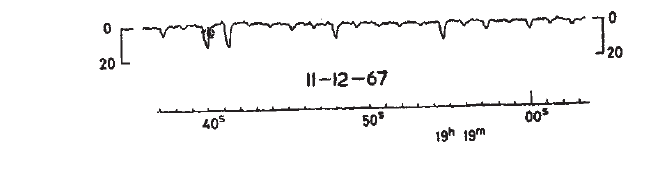
\includegraphics[width=0.6\textwidth]{pics/intro/pulses.png}
  \caption[A record of pulsating radio source]{A record of the pulsating radio
    source discovered in 1967 \citep{hewish_observation_1968}}
  \label{fig:pulse}
\end{figure}

More pulsars were soon discovered, e.g.\ the Vela with a period of
$89\,\mathrm{ms}$ \citep{large_pulsar_1968} and the Crab with a period of
$33\,\mathrm{ms}$ \citep{lovelace_pulsar_1968}. Slowing down of the periods were
also discovered in the known pulsars. The spin-down luminosity can be easily
estimated given the period and period derivative of the pulsar:
\begin{equation}
  \label{eq:spindown-power}
  L_{d} = -I\Omega\dot{\Omega} = 4\pi^2 I\frac{\dot{P}}{P^3}
\end{equation}
which works out to be $\sim 10^{39}\,\mathrm{erg/s}$ for the Crab pulsar, which
has $P = 33\,\mathrm{ms}$ and $\dot{P} = 4.2\times 10^{-13}\,{s\;s^{-1}}$. This
matches the observed luminosity of the Crab nebula, and a model was soon
proposed by \citet{gold_rotating_1969} that gas was liberated from the star and
accelerated to relativistic energies, forming a corotating magnetosphere around
the star up to the radius where corotation speed becomes equal to the speed of
light, $R_\mathrm{LC} = c/\Omega$. This radius is called the light-cylinder
radius. In this model, the relativistic gas carry away most of the spin-down
luminosity, and make its contribution to the luminosity of the nebula.

The spin-down of the pulsar was typically modeled by a spinning magnetic dipole
in vacuum. A magnetic dipole of strength $\mu$ will lose energy at a rate:
\begin{equation}
  \label{eq:dipole-spin-down}
  L_{d} = \frac{2}{3}\frac{\mu^2\Omega^4}{c^3}
\end{equation}
therefore one can naively estimate the surface magnetic field by equating this
with the spin-down luminosity \eqref{eq:spindown-power}
\begin{equation}
  \label{eq:surface-B-field}
  B_0 = 3.2\times 10^{19}\sqrt{P \dot{P}}\,\mathrm{G}
\end{equation}

For typical pulsar parameters, this gives a polar magnetic field of the order
$\sim 10^{12}\,\mathrm{G}$. The strong magnetic field required rules out the
possibility of a white dwarf, and since then a rapid rotating neutron star has
been the standard model for a rotation-powered pulsar. Equation
\eqref{eq:surface-B-field} remains the standard formula for estimating the surface
magnetic field of a newly discovered pulsar.

\subsection{High-energy radiation from pulsars}
\label{sec:observ-high-energy}

Although radio emission has been the primary wavelength at which rotation
powered pulsars are studied, only a tiny fraction ($\sim 10^{-5}$) of their
spin-down power actually goes into radio emission. For young pulsars and
millisecond pulsar (MSPs), a significant fraction of their spin-down power go
into gamma-rays in the $100\,\mathrm{MeV}$--$30\,\mathrm{GeV}$ band \citep[see
e.g.][]{abdo_fermi_2010}.

\begin{figure}[h]
  \centering
  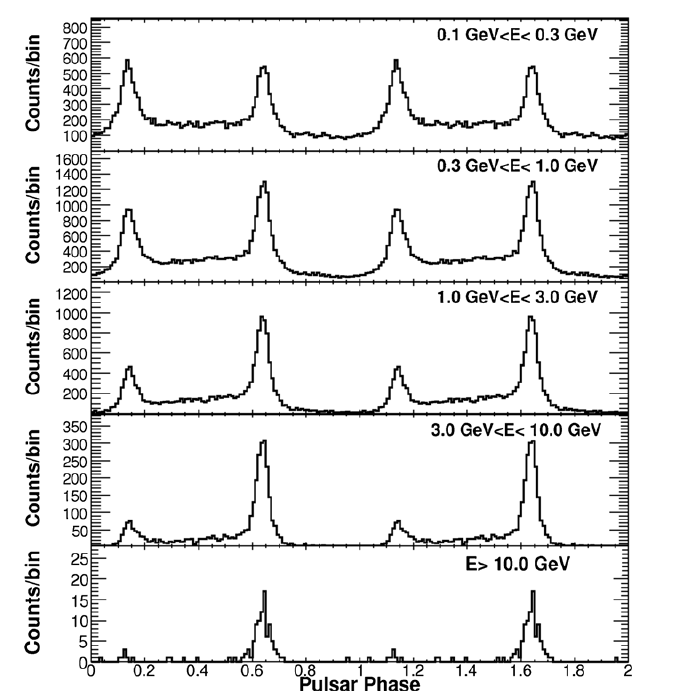
\includegraphics[width=0.7\textwidth]{pics/intro/geminga2.png}
  \caption[Gamma-ray lightcurves of Geminga]{Gamma-ray lightcurves of Geminga in
    five energy ranges, from {\it Fermi} observations
    \citep{abdo_fermi-lat_2010}.}
  \label{fig:geminga}
\end{figure}

Take the pulsar Geminga for example. It is the second brightest non-variable
$\mathrm{GeV}$ gamma-ray source in the sky. Its gamma-ray emission was first
discovered in the 70s by the SAS-2 satellite
\citep{fichtel_high-energy_1975,kniffen_distribution_1975}. In contrast to the
Crab pulsar, Geminga is observed to be radio quiet, and is the first
representative of the class of radio quiet gamma-ray pulsars. As can be seen
from figure \ref{fig:geminga}, the gamma-ray peak comes in pairs in every
period, in contrast to the typical radio peaks in rotation powered pulsars,
suggesting that the gamma-ray emission comes from very different region than
the radio emission.

After the launch of the {\it Fermi} satellite, the catalog of gamma-ray pulsars
exploded from 7 to well over 130 \citep{abdo_first_2010,abdo_second_2013}. The
gamma-ray pulsars are evenly divided into 3 groups: millisecond pulsars, young
radio-loud pulsars, and young radio-quiet pulsars. This discovery revolutionized
the way pulsars were studied. The pulsed gamma-ray emission typically carries
the highest fraction of the spin-down power $L_{d}$, therefore it can reveal the
most information about the particle acceleration and field structure in pulsar
magnetospheres, much more so than the radio emission.

Many pulsars are also found to be X-ray sources, with pulsations detected in
many of them. The emission is usually made up of two components: a thermal
component from surface cooling or heated polar caps, and a non-thermal component
that is most likely magnetospheric \citep{kaspi_isolated_2006}.


% The biggest difficulty in pulsar modeling is to account for this broadband
% radiation. A self-consistent model needs to explain not only the

\subsection{Theoretical models of the pulsar magnetosphere}
\label{sec:intro-pulsar-theory}

Despite the success of a simple vacuum dipole model, it proves to be extremely
difficult to make a more detailed self-consistent model. The vacuum dipole model
has a few problems. First is that, the electric field from uni-polar induction
effect gives a voltage that can accelerate particles to $\sim
10^{14}\,\mathrm{V}$.
% TODO: how high voltage?
This voltage has two effects: it far exceeds the binding energy of electrons and
ions at the surface of the neutron star and can extract charged particles from
the stellar surface; it also accelerates the extracted particles to energies
that produce high-energy photons that are capable of interacting with the
intense magnetic field and convert into $e^{\pm}$ pairs, thus inducing a pair
cascade \citep{erber_high-energy_1966}.

As a result, it is not possible for the pulsar magnetosphere to be near vacuum.
A minimum corotating charge density is guaranteed around the pulsar which is
conventionally called the Goldreich-Julian density \citep{goldreich_pulsar_1969}:
\begin{equation}
  \label{eq:gj-density}
  \rho_\mathrm{GJ} = -\frac{\bOm\cdot \mathbf{B}}{2\pi c}\frac{1}{1 - (\Omega r/c)^2\sin^{2}\theta}
\end{equation}
where $\theta$ is the angle between magnetic axis and the rotation axis.
% TODO: expand on the GJ model

\subsubsection{Electrosphere}
\label{sec:electrosphere}

The problem of the Goldreich-Julian model is that charge lifted from the
surface alone is not sufficient to fill the magnetosphere with
$\rho_\mathrm{GJ}$. For an aligned rotator (magnetic axis aligned with rotation
axis), there exists an electrostatic equilibrium solution for the lifted charge
\citep{jackson_new_1976, krause-polstorff_pulsar_1985,
  krause-polstorff_electrosphere_1985}. The surface charge are lifted to form a
dome around the poles of the star, and a torus near the equator. In both the
dome and the torus $\mathbf{E}\cdot \mathbf{B} = 0$, whereas an unscreened
vacuum gap exists between them (figure \ref{fig:electrosphere-intro}). This
equilibrium solution has no outgoing Poynting flux, therefore no spin-down at
all. It is a dead pulsar.

\begin{figure}[h]
  \centering
  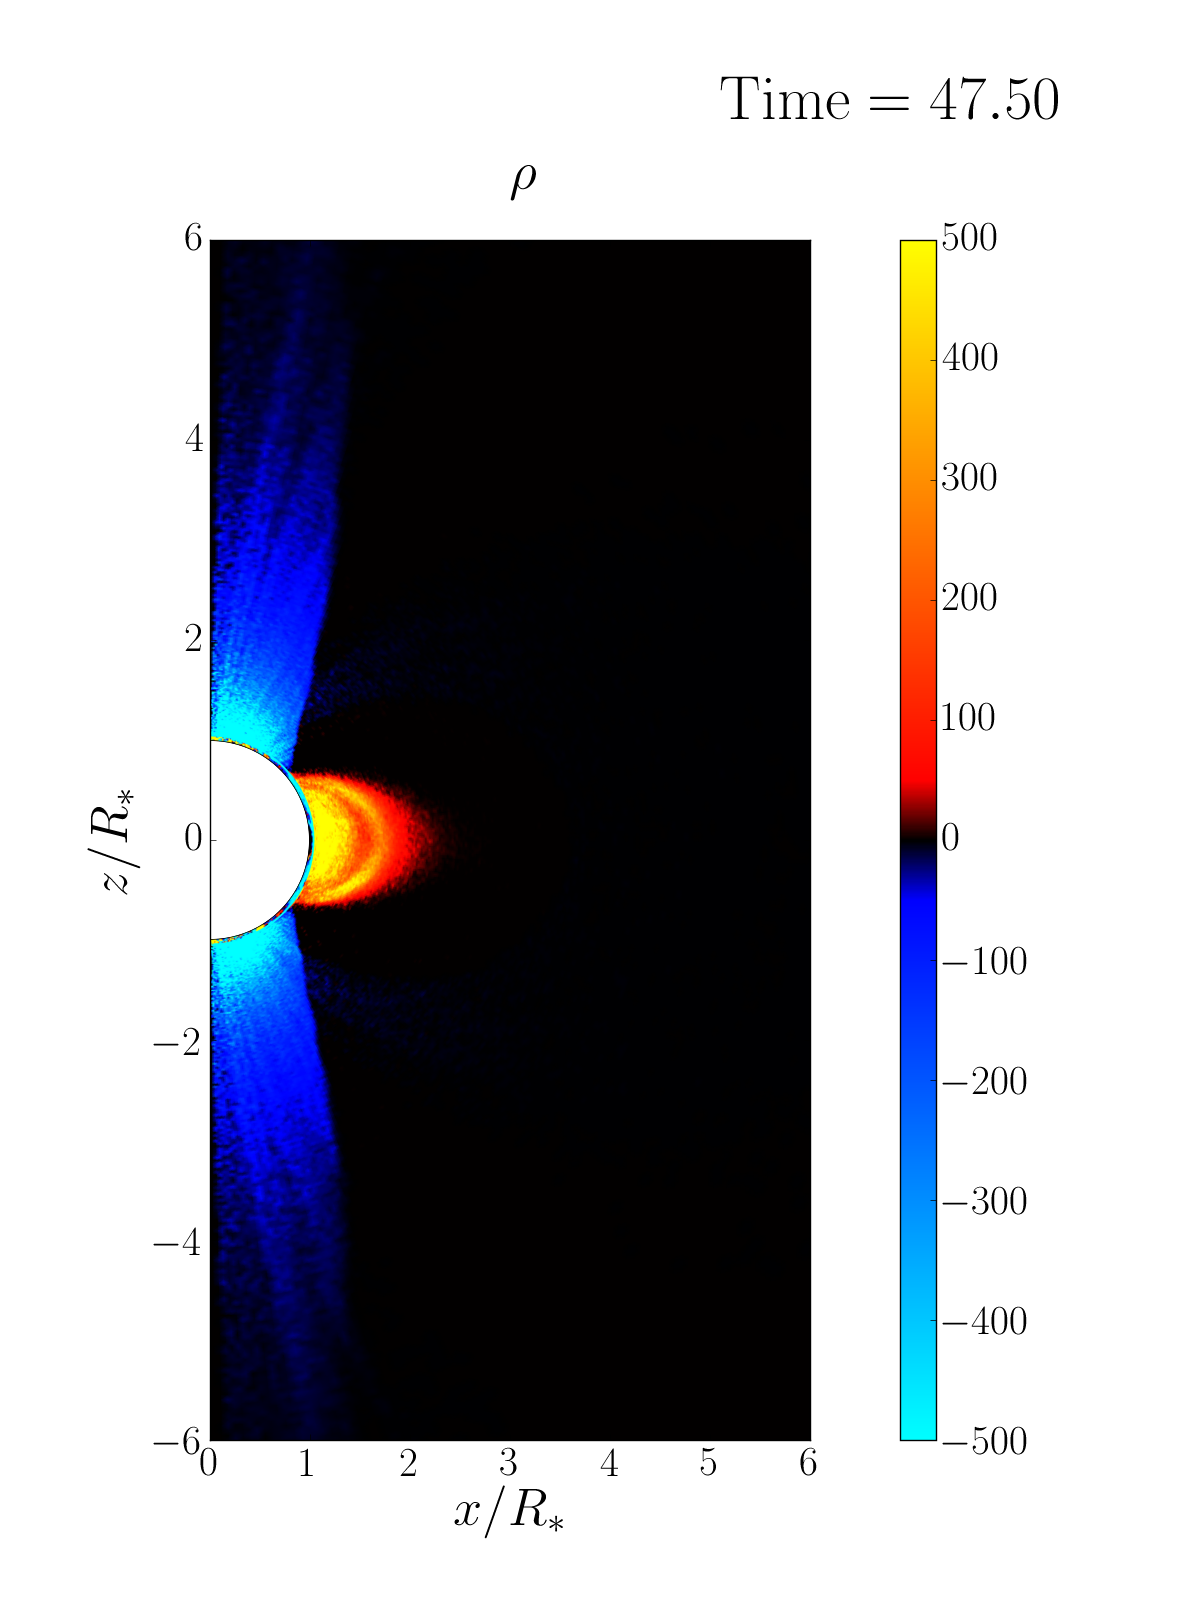
\includegraphics[width=0.6\textwidth]{pics/intro/electrosphere-new.png}
  \caption[Charge density distribution of the electrosphere of an aligned
  rotator.]{Charge density distribution of the electrosphere of an aligned
    rotator. Blue indicates negative charge and red indicates positive charge.}
  \label{fig:electrosphere-intro}
\end{figure}

It was speculated by \citet{spitkovsky_electrodynamics_2004} that oblique
rotators will be able to escape this fate due to diocotron instability
developing inside the torus, which leads to its slow expansion and eventually
reaching the light cylinder. This might jump-start the global current
circulation and allow the pulsar to start operating. But no simulation or
analytical results has been able to confirm this hypothesis. Furthermore,
\citet{petri_relativistic_2007} showed that this instability is suppressed by
relativistic effects that become important near the light cylinder.

Another problem with the electrosphere is that, a huge region with unscreened
parallel electric field exists between the dome and torus, capable of
accelerating stray particles to very high energies. These particles will be able
to produce curvature photons that are able to interact with the magnetic field
to produce $e^{\pm}$ pairs. This eventually renders the electrosphere solution
unstable to pair creation.

Pair creation in the pulsar magnetosphere has been studied extensively since the
first theoretical models of the pulsar. There are several motivations for the
pulsars to produce abundant $e^{\pm}$ outflow. One such motivation stems from
models attempting to explain the radio emission which was central to pulsar
studies for decades. Most models for radio emission involves some plasma
instability causing the clumping of charges, which requires a dense
quasi-neutral plasma. Another motivation is the observed synchrotron-radiating
$e^{\pm}$ pairs in the pulsar wind nebulae. In the case of Crab, the
multiplicity of pairs (number of $e^{\pm}$ pairs over the minimum
Goldreich-Julian density) is estimated to be $\mathcal{M} \gtrsim 10^{6}$
\citep{de_jager_gamma-ray_1996}, thus requiring the abundant pair creation in
the magnetosphere.

Therefore, particle acceleration and pair creation has been a major topic in
theoretical pulsar research for decades. One of the challenges for the models is
that pair creation is by construction a self-limiting process. The creation of
abundant neutral plasma tend to screen the accelerating electric field, thus
reducing its efficiency or even turning off the process altogether. Therefore it
is difficult to have large regions in the magnetosphere where there is
unscreened parallel electric field: all pulsar particle acceleration models
involve a somewhat local ``gap'' where unscreened electric field keeps
accelerating particles, and pairs are created outside the ``gap'', unable to
screen it.

\subsubsection{MHD and force-free models}
\label{sec:mhd-force-free}

Although the existence of gaps is crucial to fill the magnetosphere with the
required amount of plasma, it is instructive to study what happens to the
magnetosphere when plasma supply is not an issue. It makes sense to study the
approximation where plasma is so abundant as to screen all parallel electric
fields, $\mathbf{E}\cdot \mathbf{B}\approx 0$. This model assumes that the
inertial mass of the particles is much less than the magnetic field energy
$B^{2}/8\pi c$. This limit is called ``Force-free electrodynamics'' (FFE),
defined by the equation
\begin{equation}
  \label{eq:force-free}
  \rho \mathbf{E} + \frac{\mathbf{J}\times \mathbf{B}}{c} = 0
\end{equation}

Force-free electrodynamics has no constraints on the distribution of the plasma,
other than the obvious requirement that $\rho = \nabla\times \mathbf{E} / 4\pi$,
and that $\mathbf{J}$ satisfies the force-free equation \eqref{eq:force-free}.
It assumes that enough plasma is always supplied to maintain these two
conditions as demanded by the electromagnetic field.

The force-free equations together with Maxwell equations form a closed system
and can be solved for the boundary condition of a rotating neutron star. The
equations were first solved numerically by \citet{contopoulos_axisymmetric_1999}
\citetext{see also e.g.\ \citealp{goodwin_idealized_2004};
  \citealp{gruzinov_power_2005}; \citealp{timokhin_force-free_2006};
  \citealp{parfrey_introducing_2012}}. The force-free solution of the pulsar
magnetosphere shows a few interesting features:
\begin{itemize}
\item An open zone where magnetic field lines extend to infinity, $B_{\phi}\neq
  0$ and current flows along the field lines. Poynting flux $\mathbf{S} =
  \mathbf{E}\times \mathbf{B}$ points outward along the poloidal $\mathbf{B}$
  field.
\item A closed zone where $B_{\phi} = 0$ and poloidal $j=0$, filled by plasma
  with density equal to $\rho_\mathrm{GJ}$. The closed zone corotates with the
  star, similar to the torus in the electrosphere solution. Poloidal magnetic
  field remains close to dipole configuration.
\item A thin Y-shaped current sheet that separates the close and open zones,
  with the Y-point close to the light cylinder.
\end{itemize}

% TODO: Finish up the discussion for FFE, with 3D results and other stuff

However, FFE remains an approximation, and it glaringly breaks down in some
regions of the magnetosphere, namely inside the current sheets and in some
inevitable gaps where $\mathbf{E}\cdot \mathbf{B} \neq 0$ and particles are
accelerated to produce the plasma required by FFE. One can introduce finite
resistivity and use full MHD approach to study the magnetosphere % TODO: ref
. However the issue of particle acceleration and formation of localized gaps
remains impossible to tackle in this framework.

\subsubsection{Gaps and pair cascade}
\label{sec:gap-models}

Several mechanisms of forming and maintaining localized gaps where particles are
accelerated have been proposed over the years of pulsar research.

% TODO: Gap models

\section{Magnetars}
\label{sec:intro-magnetars}

% TODO: Introduce magnetars, and open up the historical observation discussions
Magnetars are a class of neutron stars with very drastic variability in X-ray
and soft $\gamma$-ray bands. They exhibit recurrent bursts, flares, and
sometimes giant bursts that can briefly outshine entire galaxies in the X-ray
luminosity. Their activity is powered by the decay of their strong magnetic
field, which is typically 100 times higher than ordinary rotation-powered
pulsars.

\subsection{Early Observations}
\label{sec:intro-magnetar-observation}

Historically ``magnetar ''was not the name given upon its discovery. The first
reports for magnetar activity can be traced back to 1979. The Venera 11 and
Venera 12 space probes recorded 3 repeated soft gamma-ray bursts from a single
source B1900+14 \citep{mazets_soft_1979}. It was believed to share similar
origins with other short gamma-ray bursts. During the same year, the space
probes also recorded hard X-ray bursts from a different source FXP 0520-66 in
Dorado, which was apparently an X-ray pulsar from the beginning
\citep{mazets_observations_1979}. These sources were designated ``Soft Gamma-ray
Repeaters'' (SGRs).

Several years later another SGR 1806-20 was found in our galaxy, and it
underwent repeated bursts on the order of 100 times over less than 10 years
\citep{kouveliotou_smm_1987,laros_new_1987}. It was also the first SGR that had
a measured spin-down rate \citep{kouveliotou_x-ray_1998}. The dipolar magnetic
field computed by the simple spin-down formula \eqref{eq:surface-B-field} gives
a surface field strength of $8\times 10^{14}\,\mathrm{G}$, much higher than
typical rotation-powered pulsars discovered yet. The ultrastrong magnetic field
of SGR 1806-20 was in line of the magnetar model proposed by
\citet{duncan_formation_1992}. In their paper they coined the term ``magnetar''
to describe young neutron stars with high magnetic field ($10^{14}\sim
10^{15}\,\mathrm{G}$), and argued that magnetars are the sources of SGRs, where
the bursts are powered by spontaneous decay of the strong magnetic field of the
magnetar. Being young objects with age $10^{3}\sim 10^{4}$ years, magnetars are
still dynamically evolving internally and build up stress that can lead to
breaking of the crust, releasing a significant amount of energy into the
magnetosphere in Alfven waves, which then powers the X-ray and soft gamma-ray
emission.

Another class of magnetars was discovered separately and recognized as
``Anomalous X-ray Pulsars'' (AXPs). In 1980 it was reported that in the
region CTB 109 there was ``an extraordinary new celestial X-ray
source'' which was a supernova remnant \citep{gregory_extraordinary_1980}. Soon
it was found that this source displays very strong pulsation with a period of
$\sim 3.5\,\mathrm{s}$ \citep{fahlman_x-ray_1981}. More X-ray pulsars were
subsequently discovered that also have similar few-second period, and share
similar soft X-ray spectra.

Thompson and Duncan speculated that AXPs may be related to SGRs, and predicted
that long-term observations of AXPs might lead to bursting behavior
\citet{thompson_soft_1996}. This was then confirmed by
observation. %TODO: flesh out this paragraph

Now both AXPs and SGRs are recognized under the same umbrella known as
magnetars. Among the $\sim 30$ known magnetars, a more intrinsic
characterization is their quiescent luminosity. {\it Transient magnetars} are
typically only detected during their bursts, while {\it persistent magnetars}
are what used to be associated with AXPs, showing up with strong X-ray
pulsations.

\subsection{Observational Puzzles}
\label{sec:magnetar-puzzles}

For transient magnetars, apart from short and irregular bursts that are the
signature of SGR activity, they also show large outbursts with short rise time
and long decay. A classic example is the transient magnetar XTE J1810-197, which
underwent an outburst in early 2013 \citep{ibrahim_discovery_2004}, and its
luminosity slowly decayed to quiescent levels over several years (figure
\ref{fig:outburst-light-curve}). \citet{gotthelf_anatomy_2007} found that the
X-ray spectrum of the magnetar during outburst can be fitted by 2 blackbody
components, one with lower temperature and larger area, which subsequently cooled
but expanded to cover almost the entire star, and another with smaller area and
higher temperature, and {\it shrinking} over time (figure \ref{fig:shrinking-hotspot}).

\begin{figure}[h]
  \centering
  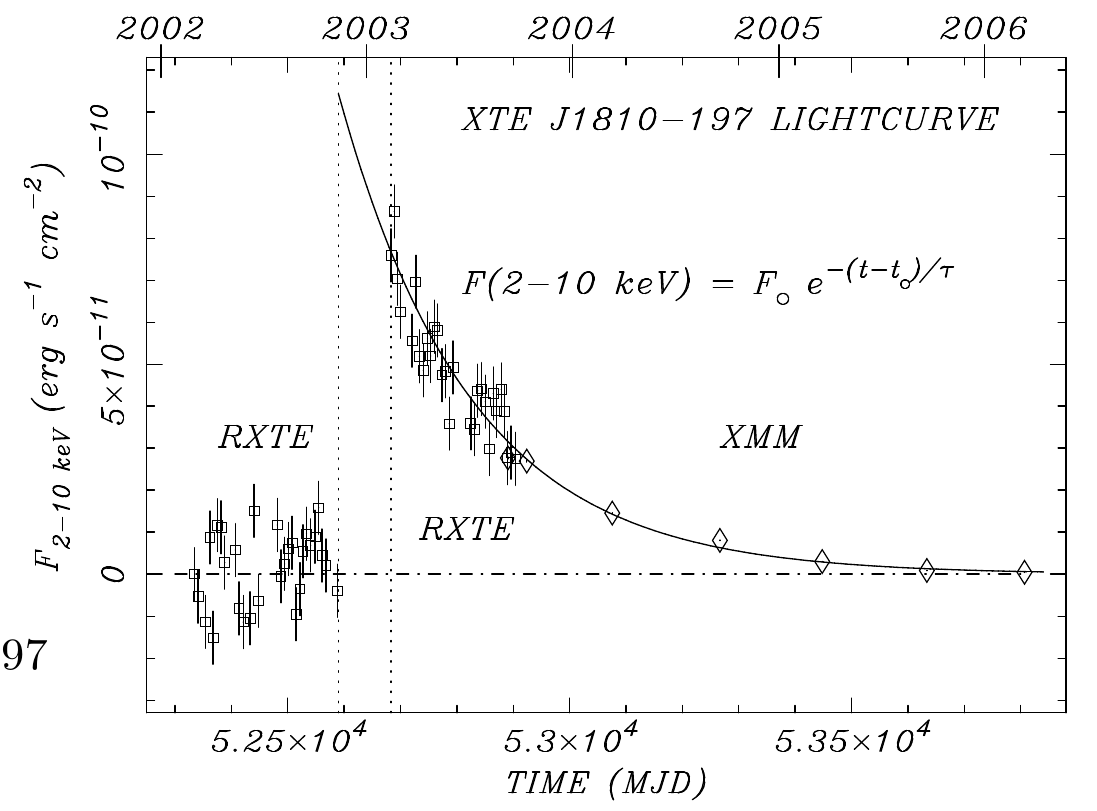
\includegraphics[width=0.7\textwidth]{pics/intro/transient.png}
  \caption[Light curve for the outburst from transient magnetar XTE J1810-197]{Light curve for the outburst from transient magnetar XTE J1810-197 \citep{gotthelf_anatomy_2007}.}
  \label{fig:outburst-light-curve}
\end{figure}

\begin{figure}[h]
  \centering
  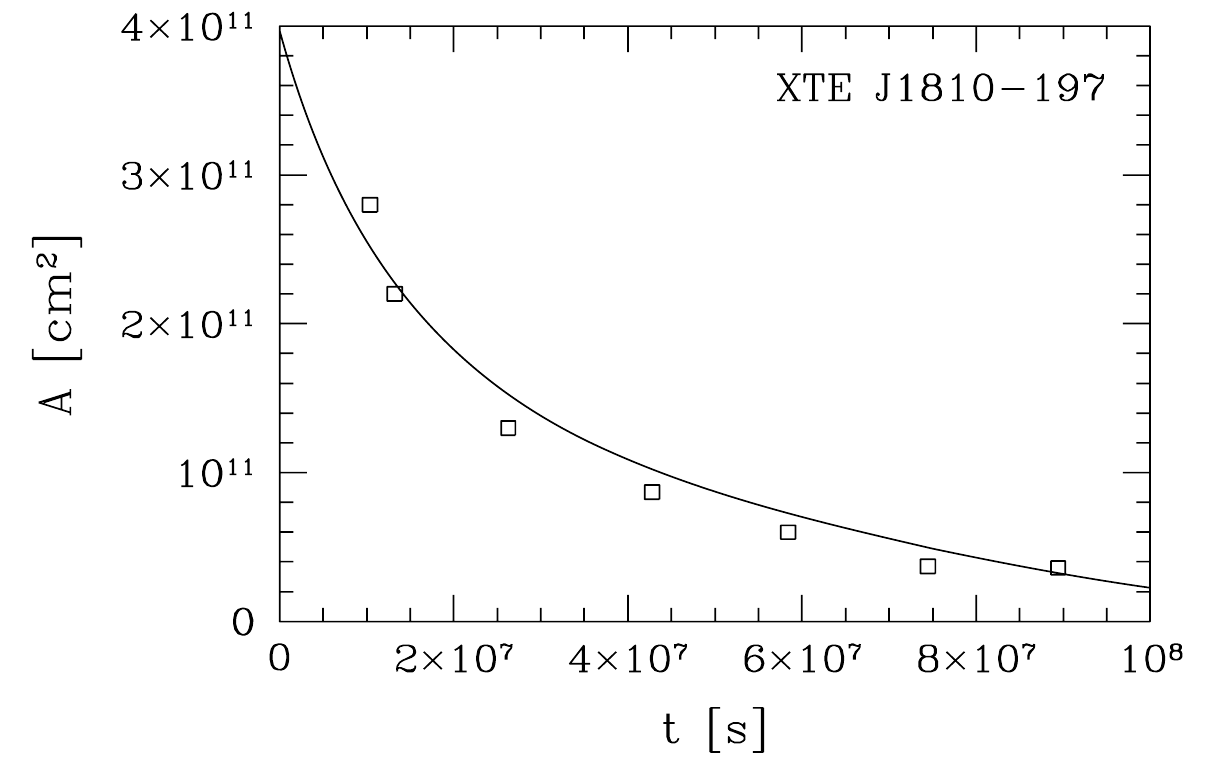
\includegraphics[width=0.7\textwidth]{pics/intro/shrink-spot.png}
  \caption[Evolution of the fitted area of the hot component in the X-ray
    spectrum of XTE J1810-197.]{Evolution of the fitted area of the hot component in the X-ray
    spectrum of XTE J1810-197. The area shrunk by a factor of more than 8 over
    the course of a few years.}
  \label{fig:shrinking-hotspot}
\end{figure}

The shrinking hotspot feature was not only seen in one transient magnetar.
Figure \ref{fig:hotspots} shows the evolution of luminosity versus the area of
the fitted hotspot for 7 of the known transient magnetars for which a hotspot
has been identified. All seem to follow a similar trajectory over the $A$-$L$ plane.

\begin{figure}[h]
  \centering
  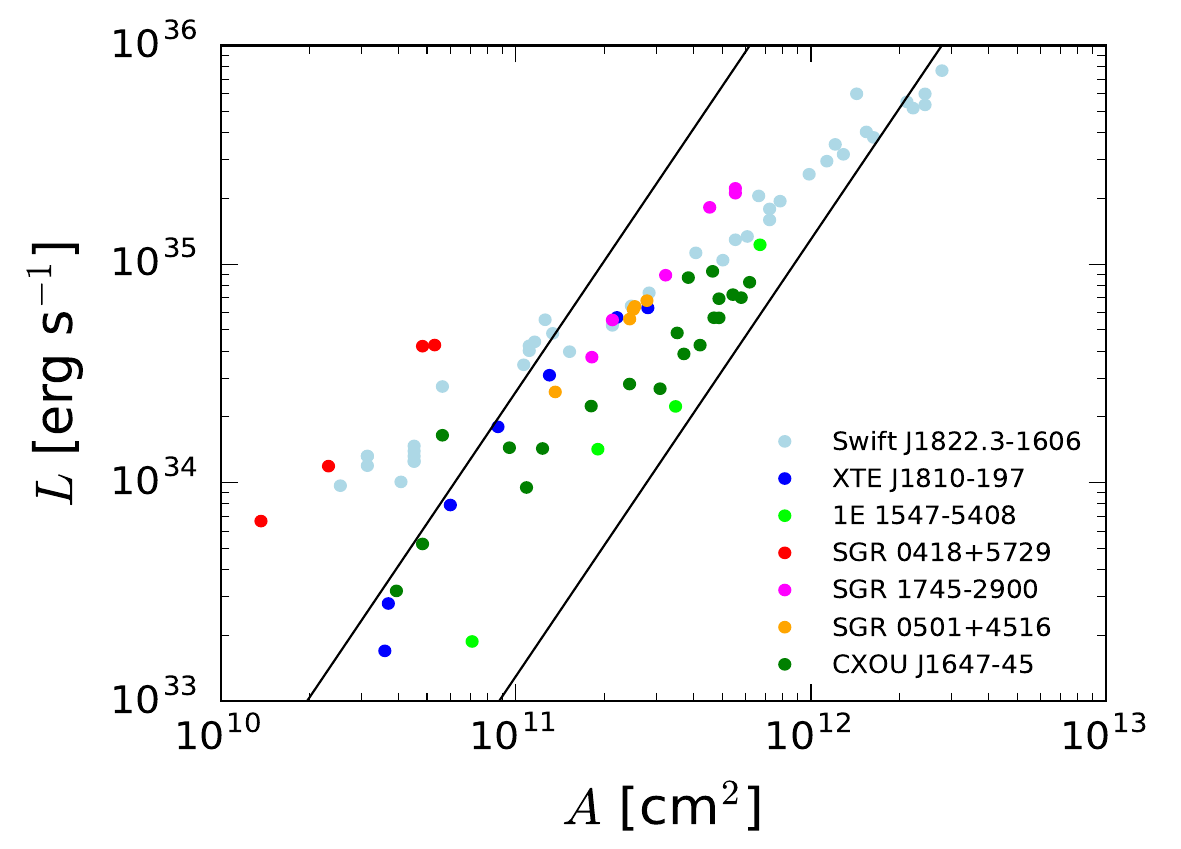
\includegraphics[width=0.7\textwidth]{pics/intro/hot-spot.png}
  \caption[The evolution of hotspots observed on transient magnetars following
    outbursts.]{The evolution of hotspots observed on transient magnetars following
    outbursts. The hotspots shrink and become dimmer over time, tracking a
    similar trajectory on the $A$-$L$ plane. \citep{beloborodov_magnetar_2016}}
  \label{fig:hotspots}
\end{figure}

% TODO: Fill this part

The


\subsection{Theoretical Models}
\label{sec:intro-magnetar-theory}

Here describe the crustal shear and magnetospheric twist model. Describe the
particle flow, acceleration. Double layer. Resonant scattering. Go into more
detail in the appendix.

\section{This Dissertation}
\label{sec:intro-outline}

In this dissertation we will attempt to address the problem of particle
acceleration and global structure of the magnetosphere of pulsars and
magnetars.

Chapter \ref{chap:pic} will be devoted to a detailed introduction of the
particle-in-cell technique, which will be the basic numerical tool for our
study.

Chapter \ref{chap:polar-cap} will focus on a local study of the pulsar
polar cap. We will look at the region well within the pulsar magnetosphere, and
approximate the geometry as 1D. We will discuss implications of this
approximation, and what we can and can not learn from this local study.

Chapter \ref{chap:pulsar} will study the global pulsar magnetosphere, motivated
by the study of the polar cap particle acceleration.

Chapter \ref{chap:magnetar} will study the twisted magnetosphere of magnetars.

Chapter \ref{chap:explorations} will contain some exploratory extensions of the
PIC code in the hope of tackling practical physical problems.

% Local Variables:
% TeX-master: "../thesis"
% zotero-collection: #("16" 0 2 (name "Thesis"))
% End:
